\section{Visual Object Tracking Datasets}

% ##############################################################################
\subsection{KITTI Object Tracking}
\label{ssec:DatasetKITTIObjectTracking}

This object tracking benchmark~\cite{geiger2012cvpr} consists of $21$ training sequences and $29$ test sequences. Even though there have been labeled $8$ different classes, only the classes ``car'' and ``Pedestrian'' are evaluated in this benchmark, as only for those classes enough instances for a comprehensive evaluation have been labeled. Considering our potential traffic application, this fact does not represent a disadvantage. The goal of the object tracking task in this benchmark is to estimate object tracklets for the classes ``car'' and ``pedestrian''. Only $2D$, axis-aligned \glspl{bbox} in each image are evaluated.

% ##############################################################################
\subsection{MOT17}
\label{ssec:DatasetMOT17}

\motseventeen{}~\cite{dendorfer2020motchallenge} is probably the most commonly utilized benchmark for evaluating \gls{mot} trackers. This challenge contains seven different indoor and outdoor scenes of public places with pedestrians as objects of interest. Each video corresponding to one scene is divided into two clips, one for training and the other for testing. However, there are three different versions of detections available produced by three different object detectors, thereby tripling the number of available videos in terms of distinct annotations. This benchmark challenge accepts both online and offline tracking approaches.

% ##############################################################################
\subsection{UA-DETRAC}
\label{ssec:DatasetUADETRAC}

The most important benchmark dataset for our work is \uadetrac{}~\cite{wen2020uadetrac}. To the best of our knowledge, this dataset most favorably suits the needs of all surveyed datasets available. The primary reason is that it provides a plethora of traffic situations recorded using a static camera (\figtext{}~\ref{fig:DatasetUADETRAC}). This work provides high-quality human-generated annotations with a lot of additional information about the captured vehicles, such as the intensity of their occlusion.

\uadetrac{} is considered a challenging real-world multi-object detection and multi-object tracking benchmark. The dataset consists of $10$ hours of videos captured at $24$ different locations in China. The videos are recorded at $25$ \gls{fps}, with resolution of $960 \times 540$ pixels. There are more than $140\ 000$ frames and $8\ 250$ vehicles that are manually annotated, leading to a total of $1.21$ million labeled \glspl{bbox} of objects.

% ------------------------------------------------------------------------------
\begin{figure}[t]
    \centerline{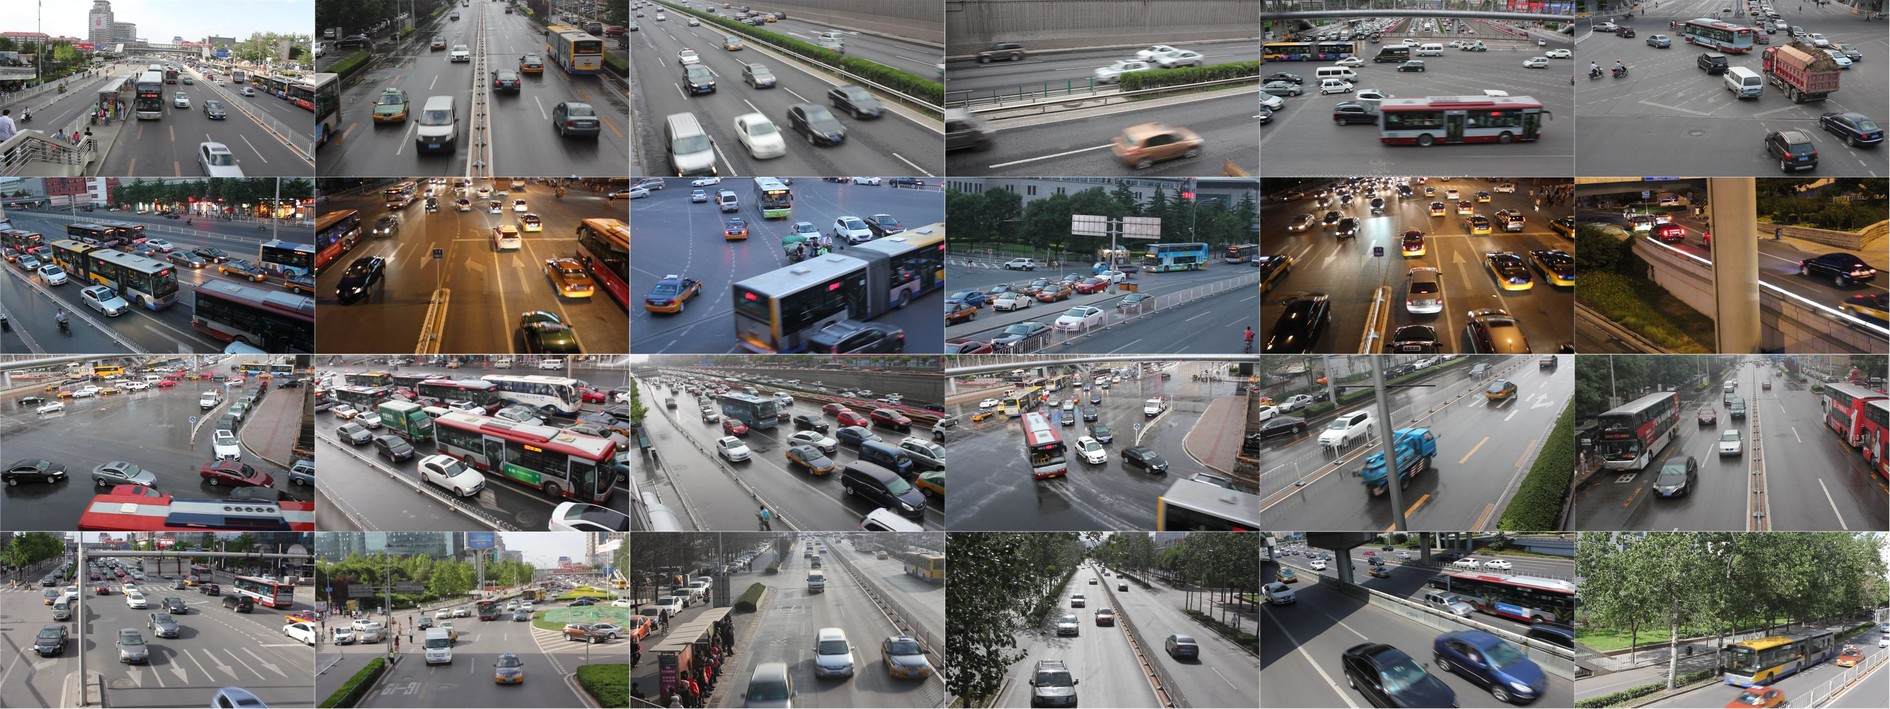
\includegraphics[width=\linewidth]{figures/datasets/uadetrac_samples.jpg}}
    \caption[\uadetrac{} dataset]{A sample from the \uadetrac{} dataset. The whole dataset consists of diverse traffic situations captured using a static camera viewed from various angles. \externalsrc{\cite{wen2020uadetrac}}}
    \label{fig:DatasetUADETRAC}
\end{figure}
% ------------------------------------------------------------------------------

\def\uadetracfigsize{0.4}

% ------------------------------------------------------------------------------
\begin{figure}[t]
    \centering
    \begin{subfigure}[b]{\uadetracfigsize\textwidth}
        \centering
        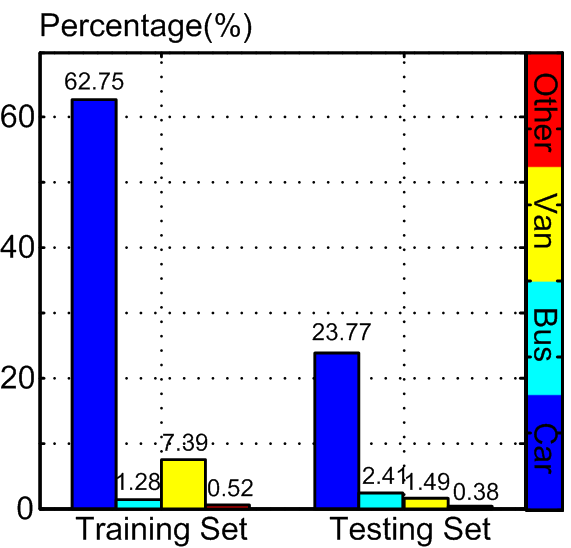
\includegraphics[width=\textwidth]{figures/datasets/uadetrac_stats_vehicle_category.png}
        \caption[]{}
    \end{subfigure}
    \hfill
    \begin{subfigure}[b]{\uadetracfigsize\textwidth}
        \centering
        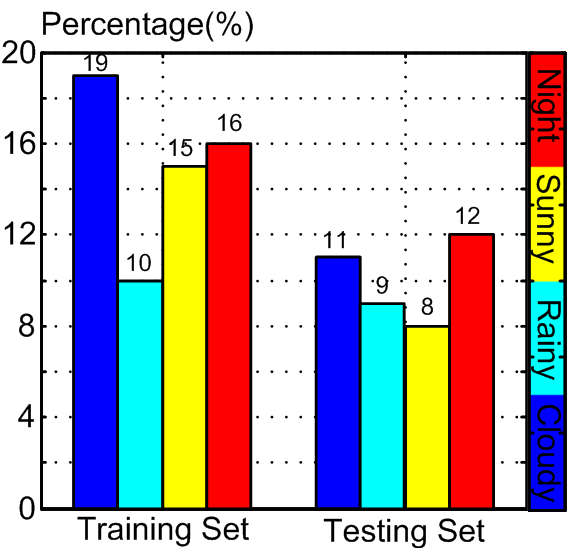
\includegraphics[width=\textwidth]{figures/datasets/uadetrac_stats_weather.png}
        \caption[]{}
    \end{subfigure}
    \hfill
    \begin{subfigure}[b]{\uadetracfigsize\textwidth}
        \centering
        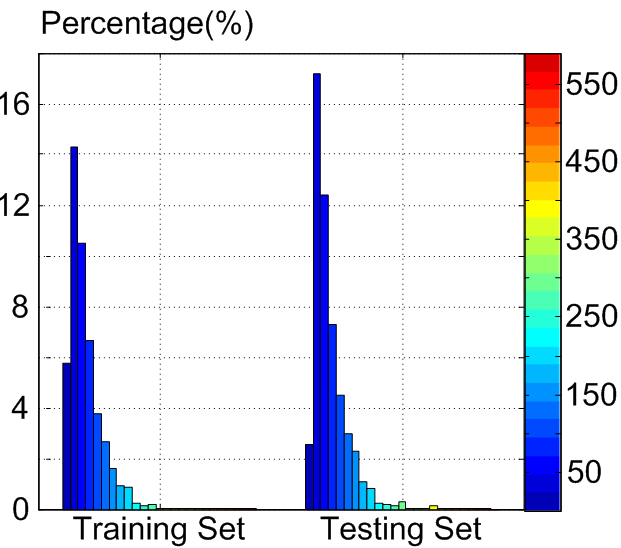
\includegraphics[width=\textwidth]{figures/datasets/uadetrac_stats_scale.png}
        \caption[]{}
    \end{subfigure}
    \hfill
    \begin{subfigure}[b]{\uadetracfigsize\textwidth}
        \centering
        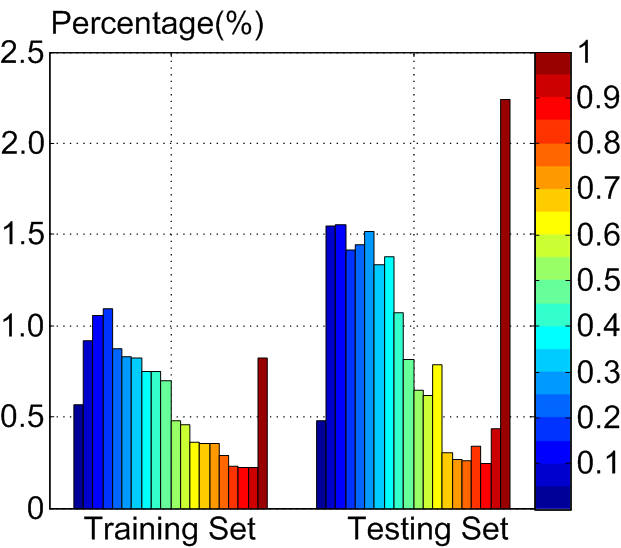
\includegraphics[width=\textwidth]{figures/datasets/uadetrac_stats_occlusion_ratio.png}
        \caption[]{}
    \end{subfigure}
    \caption[\uadetrac{} dataset overview]{Summary statistics of the \uadetrac{} dataset. \imgpartdesc{a} shows the distribution of vehicle categories, one of \emph{car}, \emph{bus}, \emph{van} or \emph{other}; \imgpartdesc{b} shows the varying weather conditions belonging to either \emph{night}, \emph{sunny}, \emph{rainy} or \emph{cloudy}; \imgpartdesc{c} depicts the change in scale given by the square root of the \gls{bbox} pixel area; and \imgpartdesc{d} reflects the occlusion ratio throughout the dataset computed as the fraction of the vehicle \gls{bbox} being occluded . \externalsrc{\cite{wen2020uadetrac}}}
    \label{fig:UADETRACStats}
\end{figure}
% ------------------------------------------------------------------------------

Since this dataset is of paramount importance to our research, here we provide more details about the structure and properties of the contained data compared to other datasets described in our work. The dataset consists of $100$ videos, where $60$ of them are dedicated to training, while the remaining $40$ are used for testing. Ground-truth annotations are provided in both variations. This is not always the case, as several benchmarks do not disclose annotations for the test dataset, \egtext{}, \datasetname{KITTI}~\cite{geiger2012cvpr}.

The authors provide extensive information about the vehicle, including its speed in \gls{fps}, color, orientation, and occlusion. The dataset contains numerous scenes where the number of cars is very high. More specifically, some basic statistical properties of the distribution of the number of cars throughout the dataset are: mean $9.21$, standard deviation $6.60$, median $21$, and maximum $49$. The data were obtained by collecting the number of annotated cars for each frame.
